\section{Entities}\label{sec:01}
In order to access the Bakery System, You should be registered as a User therein. 
After the registration a User can log in to the system using their username and password. 
% 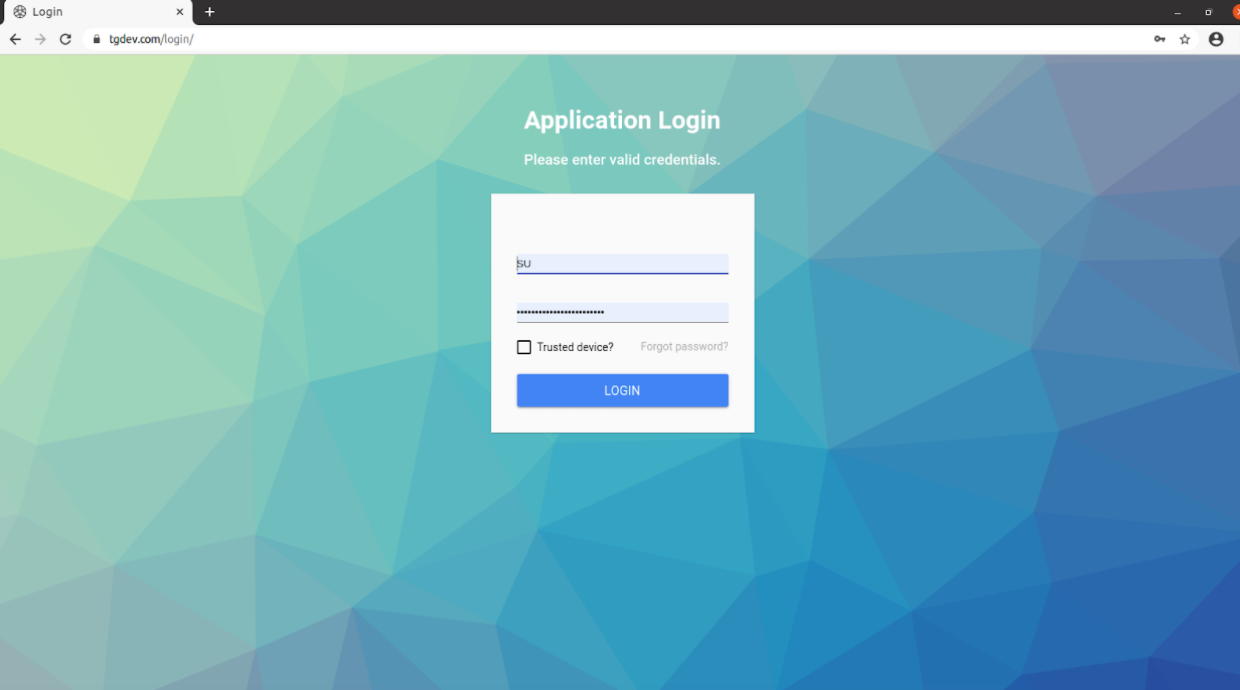
\includegraphics[height=5cm]{login.png}\\

The System consists of multiple entities - key players in the system, which are used.

You can review them by clicking on :
% \includegraphics[height=5cm]{review.png}\\

Depending on the role a user has in the system, they can either have the ability to register and edit some entities or not. 
The key entities are:

- Person 

- Manager

- Carrier

- Location

- Order

- Product

- Employment

- OrderItem

\subsection{Person}
A person represents an entity that is any person (they can be either one of the workers in a bakery or just a person).

% 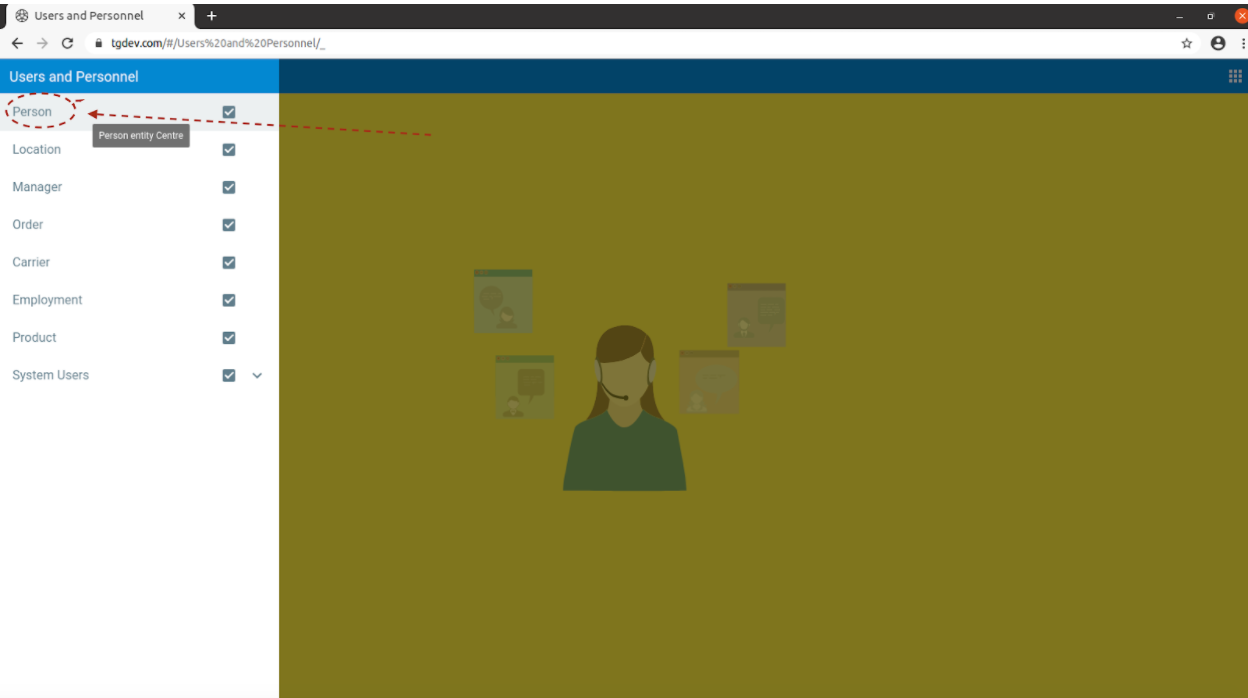
\includegraphics[height=5cm]{person1.png}\\
Creation of a new Person.

% 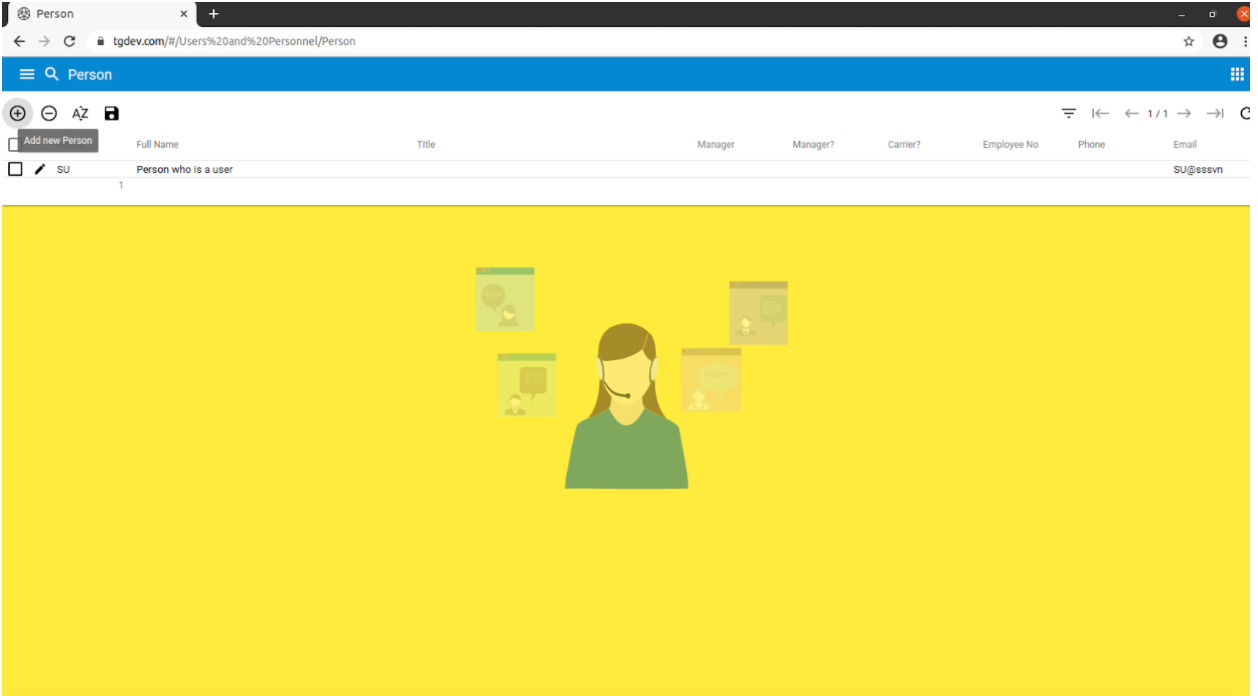
\includegraphics[height=5cm]{person2.png}\\
To create a new person you need to  fill in the important fields such as:
% 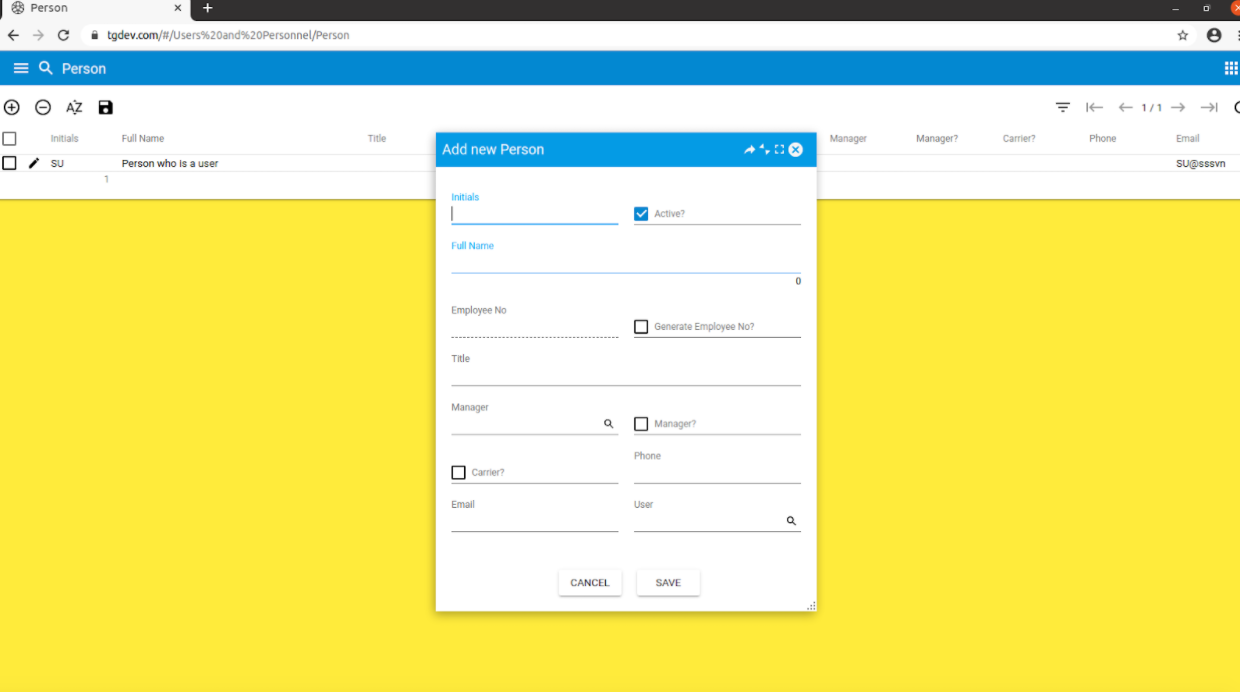
\includegraphics[height=5cm]{person3.png}\\

- Initials →  required, string, spaces are not allowed in the initials

- Active → required, the indicator of an active participant in the system. The environment cannot interact with inactive Person.

- Title →  optional, person’s position.

- Employee Number → optional,  the indicator number of the employee, is generated automatically, if specified in the checkbox to the right, then position must be specified as well. 

- Phone number → optional String, phone number of a Person

- Email →  optional, String, email

- aManager →  optional, Manager of this employee

- Manager? →  optional checkbox, indicates whether this employee is in the manager role

- Carrier? → optional checkbox, indicator of whether this Person is a carrier

- User → optional, a system user associated with this Person

You can search for a Person using the following properties: 
% 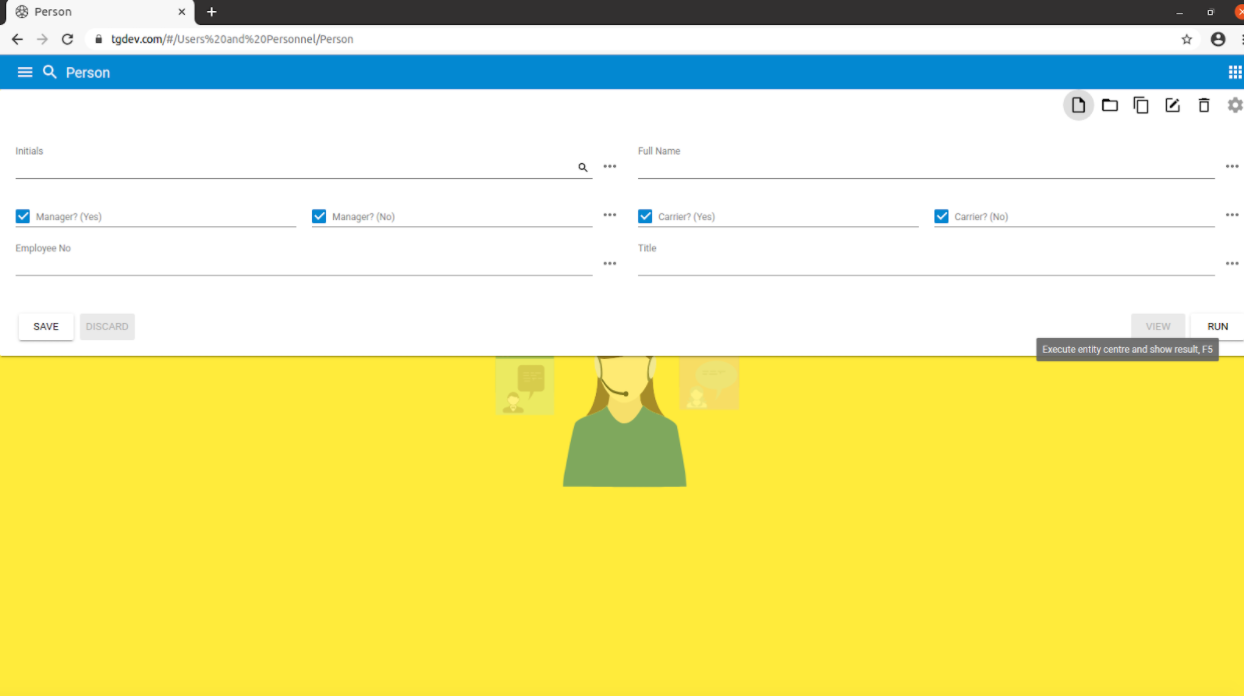
\includegraphics[height=5cm]{person4.png}\\

